\documentclass[lettersize,journal]{IEEEtran}
\usepackage[acronym]{glossaries}
\usepackage{amsmath,amsfonts}
\usepackage{algorithmic}
\usepackage{algorithm}
\usepackage{array}
\usepackage[caption=false,font=normalsize,labelfont=sf,textfont=sf]{subfig}
\usepackage{textcomp}
\usepackage{stfloats}
\usepackage{url}
\usepackage{verbatim}
\usepackage{graphicx}
\usepackage{cite}
\hyphenation{op-tical net-works semi-conduc-tor IEEE-Xplore}
% updated with editorial comments 8/9/2021

% Load acronyms
\loadglsentries{acronyms}

\begin{document}

\title{MQTT-Discovery and UPnP: \\a comparison}

\author{\IEEEauthorblockN{Daniele Foschi} \\
\IEEEauthorblockA{\textit{Alma Mater Studiorum Università di Bologna} \textit{UNIBO}\\
Bologna, Italy \\
daniele.foschi2@studio.unibo.it\\
https://github.com/DaniDF/MQTT-Discovery-vs-UPnP}
}

% The paper headers
%\markboth{Journal of \LaTeX\ Class Files,~Vol.~14, No.~8, August~2021}%
%{Shell \MakeLowercase{\textit{et al.}}: A Sample Article Using IEEEtran.cls %for IEEE Journals}

\maketitle

\begin{abstract}
TODO 
\end{abstract}

\begin{IEEEkeywords}
MQTT, discovery, upnp, project activity.
\end{IEEEkeywords}

\section{Introduction}
% * Descrizione alto livello dispositivo IoT
% * Cosa sono gli protocolli di discovery e a cosa servono
% * Definizione di UPnP e MQTT evidenziando le differenze
% * Obiettivo del progetto
% * Cosa è stato fatto
% * Breve frase sui risultati ()
% * Remainder off (descrivere il contenuto delle sezioni sucessive)

\gls{iot} has a lot of definitions: from International Telecommunication Union is \textit{"A global infrastructure for the information society, enabling advanced services by interconnecting (physical and virtual) things based on existing and evolving interoperable information and communication technologies"}. IEEE defines \gls{iot} as a list of features:

\begin{itemize}
    \item A network
    \item Objects are identifiable as things with unique identifiers
    \item When a thing communicate should use internet at least in one segment of the communication
    \item Things can have sensing or actuating or both capabilities
    \item They should be programmable as result of injection of intelligence
    \item The offered services should be available anywhere, anytime and for anything
\end{itemize}

In a environment populated by a large variety of different devices with different needs and capabilities designing a standard useful for communicating with them is a challenge.
Discovery protocols are designed to reconcile the dichotomy between the requirement for highly specific, ad-hoc protocols capable of granular device control and the necessity for generalized frameworks that can accommodate a highly heterogeneous ecosystem of devices.
By employing these protocols, an \gls{iot} device achieves autonomous configuration through active participation in the advertisement and solicitation of network-based services.
Devices functioning as service providers systematically broadcast their available resources, the specific services they offer, and the requisite operational guidelines for invocation, such as the appropriate \gls{api}. Furthermore, discovery protocols streamline the connectivity paradigm between clients and target resources or services. 
Consequently, this architecture ensures that clients are adequately equipped to transmit necessary input parameters to the services and successfully retrieve the corresponding computational results.

In particular this dissertation is focused on \gls{upnp} and a protocol based on \gls{mqtt} knwon as \gls{mqttd}. \gls{upnp} is a discovery protocol without infrastructural nodes where each node can advertise and listen for services. In particular nodes that make available services are called \textit{devices} and those searching for services are called \textit{control-points}.
In \gls{mqttd} there is a third entity called \textit{broker} that facilitates the communication between services and clients.

This dissertation wants to highlight the performance differences between \gls{upnp} and \gls{mqttd} in \gls{iot} environment. The main focus is measuring and comparing latency and robustness in different deployment configurations: how different amount of data producers and consumers affect the protocol performances.

%TODO frase sui risultati

%TODO remainder

\section{Discovery protocols for IoT}
% * Definizione di discovery per IoT
% * Descrivere i protocolli (con immagini)
% * Descrizione del problema

Resource discovery protocols can be categorised into: centralised and distributed. In centralised approaches such as \gls{mqtt}, resources are registered in a directory that serves as intermediary between providers and users. In distributed approaches such as \gls{upnp}, users discover active resources through direct communication with resources in a \gls{p2p} fashion with no need for an intermediary directory \cite{comp_ana_disc}.

\gls{upnp} is a \gls{p2p} discovery service without hierarchical structuring.
In \gls{upnp} two entities can be distinguished: \textit{control-point} the entity that look for services and resources and \textit{device} the entity that make services available.
A device can dynamically join a network and obtain a locally valid \textit{IP} address. After it can make its capabilities visible and discover others, if present, and dynamically leave the network.
\gls{upnp} uses \textit{XML} for the description of the resources, services and action invocations. 

\begin{figure}[!ht]
    \centering
    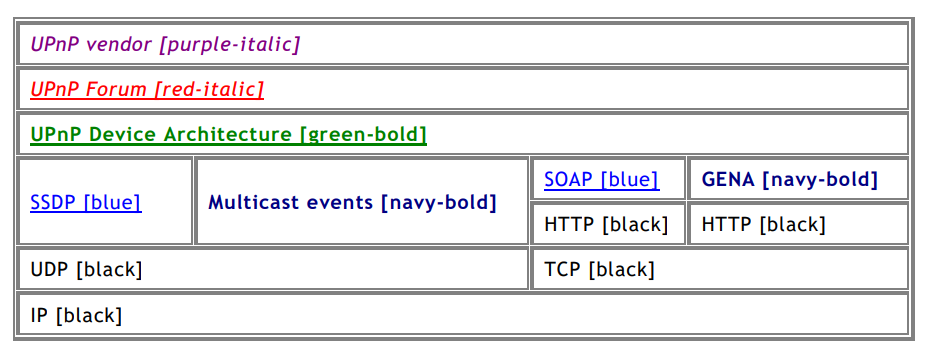
\includegraphics[width=1\linewidth]{results/upnp_protocol_stack.png}
    \caption{UPnP Protocol Stack \cite{ocf_upnp_architecture_2020}}
    \label{fig:upnp_prtocol_stack}
\end{figure}

\gls{upnp} can be divided into 4 parts: \gls{ssdp}, \gls{http}, \gls{soap} and \gls{gena}.
\gls{ssdp} is a network protocol based on the Internet protocol suite for advertisement and discovery of network services and presence information. It is a text-based protocol based on a non fully compliant version of \gls{http} over UDP \cite{ocf_upnp_architecture_2020}.
\gls{soap} is a messaging protocol specification for exchanging structured information in XML message format. In \gls{upnp} it is used by the \textit{control-point} for requesting the execution of services with specified arguments on the \textit{device} and by the \textit{device} for returning the results.
\gls{gena} is an event notification protocol used by \textit{devices} to publish variables updates to subscribed \textit{control-points}. \gls{gena} supports both unicast and multicast event notification.

\gls{mqttd} is a discovery protocol based on \gls{mqtt}. \gls{mqtt} is a lightweight publish-subscribe messaging protocol designed for constrained devices. \gls{mqttd} is a metadata‑exchange convention built on top of the \gls{mqtt} protocol that standardises how devices and services describe themselves and publish their configuration to an \gls{mqtt} broker. It enables automatic detection, registration, and integration of devices in home‑automation or IoT ecosystems without requiring manual configuration.

This dissertation aims to evaluate the performance of \gls{mqttd} and \gls{upnp} in deployments with different number of deployed devices and different number of control devices. For \gls{mqttd} will be evaluated how the performances changes with respect to the requested \gls{qos}.
The evaluated metrics for this study are latency and robustness. The first wants to measure the time needed for discovery and the execution of the first interaction between \textit{control-point} and \textit{device}. The second wants to measure the ratio between the discovered devices and the actual deployed devices.

\section{Implementation}
% * Descrivere il fatto di aver implementato UPnP/MQTT
% * Mettere descrizione dei componenti software dei protocolli
% * Differenze rispetto allo standard (MX non limitato a 5)
% * Motivare la scelta delle tecnologie

In order to implement a testing environment a fully compatible \gls{upnp} \textit{device} and \textit{control-point} were implemented based on the official documentation \cite{ocf_upnp_architecture_2020}. All its parts were implemented: \gls{ssdp}, \gls{soap}, \gls{gena}. For \gls{http} the standard library already available in Go Lang is used.
In order to demonstrate compatibility based on the standard a third part \gls{upnp} client (only) library is used \cite{goupnp}.

For \gls{mqttd} a already available implementation of \gls{mqtt} is used and was implemented only a wrapper for the \gls{mqttd} data format. As \gls{mqtt}-Broker Mosquitto is chosen as one of the most popular broker in IoT deployments.

All the software components implemented by the author are written in Go Lang for maximising efficiency but still using a higher level programming language.

\section{Experimental results}
% * Sintesi obiettivo degli esperimenti
% * Come fatto setup
% * Foto setup sperimentale

The experiments were conducted in a real closed network where only the testing equipment were connected. All the experiments were run both wireless using IEEE802.11n and cabled. During the tests were deployed 1, 2, 3, 4, 5, 6, 7, 8, 9, 10, 20, 30, 40, 50, 60, 70, 80, 90, 100 devices and control-points in all the possible values combinations. In case of \gls{mqtt} each combination were tested for \gls{qos} 0, 1 and 2. Also each combination were tested 30 times and the results are averaged in order to minimise statistical fluctuations.

In \gls{ssdp} every time a node wants to discover a \textit{device} sends a $\text{M-SEARCH}$ request asking if a device is present with some described characteristics. As soon as a \textit{device} receives the request and confirms that it is compliant with the requested device it sends back a response. Since the number of responses can not be predicted the \textit{control-point} add to the search request the parameter $\text{MX}$. This parameter indicates the maximum value of seconds that the \textit{control-point} waits for the response. A \textit{device} that need to respond to a request has to wait a random number of milliseconds between 0 and the value specified by $\text{MX}$. In this way a possible \gls{dos} done through the flooding of the network of responses is mitigated \cite{ocf_upnp_architecture_2020}.

The experiments tried to evaluate the effectiveness of the $\text{MX}$ parameter by removing the random wait time from the \textit{device} response.

In the following subsections present the measured metrics for values 1, 5, 10, 50, 100 but a more detailed verision can be find in appendix \ref{apx_more_dta_points}.

\subsection{Lantency comparison}
%\begin{itemize}
%    \item Espandere obiettivo test (motivazione)
%    \item Descrizione esperimento (metodi)
%\end{itemize}

\begin{figure}[!h]
    \subfloat[]{
\includegraphics[width=1.61in]{results/upnp_latency_light.png}%
    \label{fig_upnp_latency_light}}
    \hfill
    \subfloat[]{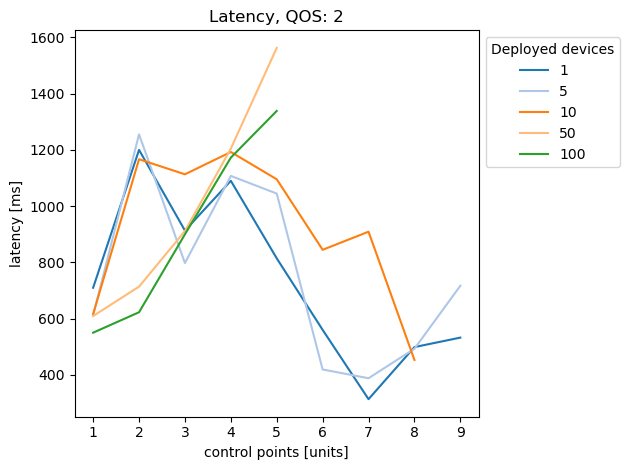
\includegraphics[width=1.61in]{results/mqtt_latency_q2_light.png}%
    \label{fig_upnp_latency_light_cabled}}
    \caption{Comparison of (a) \gls{upnp} and (b) \gls{mqtt} latency. See \ref{fig_upnp_latency} and \ref{fig_mqtt_latency_q0}, \ref{fig_mqtt_latency_q1}, \ref{fig_mqtt_latency_q2}}
    \label{fig_upnp_latency}
\end{figure}

\begin{itemize}
    \item Osservazione
\end{itemize}

Grafico 1 5 10 50 100 comparison M

\begin{itemize}
    \item Osservazione
\end{itemize}

\subsubsection{Wired vs Cabled}
\begin{itemize}
    \item Motivazione dei test
\end{itemize}

Grafico 1 10 50 comparison UvM

\begin{itemize}
    \item Osservazione
\end{itemize}

\subsection{Robustness comparison}
\begin{itemize}
    \item Espandere obiettivo test (motivazione)
    \item Descrizione esperimento (metodi)
\end{itemize}

Grafico 1 5 10 50 100 comparison U

\begin{itemize}
    \item Osservazione
\end{itemize}

Grafico 1 5 10 50 100 comparison M

\begin{itemize}
    \item Osservazione
\end{itemize}

\subsubsection{Wired vs Cabled}
\begin{itemize}
    \item Motivazione dei test
\end{itemize}

Grafico 1 10 50 comparison UvM

\begin{itemize}
    \item Osservazione
\end{itemize}

\begin{figure}[!ht]
\centering

\includegraphics[width=2.5in]{results/upnp_robustness_light.png}
\caption{Simulation results for the network.}
\label{fig_1}
\end{figure}

\section{Conclusions}
\begin{itemize}
    \item Cosa è statto fatto in breve
    \item Cosa è stato dimostrato
    \item Future directions
\end{itemize}

\printglossary[type=\acronymtype]

\newpage

\appendix
\section{More data points}
\label{apx_more_dta_points}

\subsection{\gls{mqtt}}
\subsubsection{\gls{mqtt} latency}
\begin{figure*}[!ht]
    \centering
    \subfloat[]{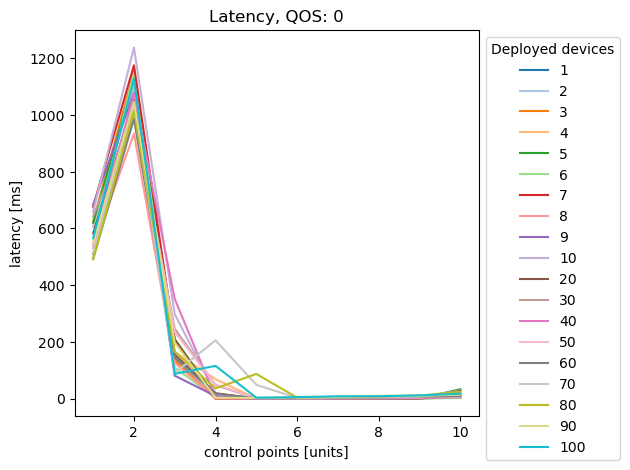
\includegraphics[width=3.5in]{results/mqtt_latency_q0.png}
    \label{fig_mqtt_latency_q0_wireless}}
    \hfil
    \subfloat[]{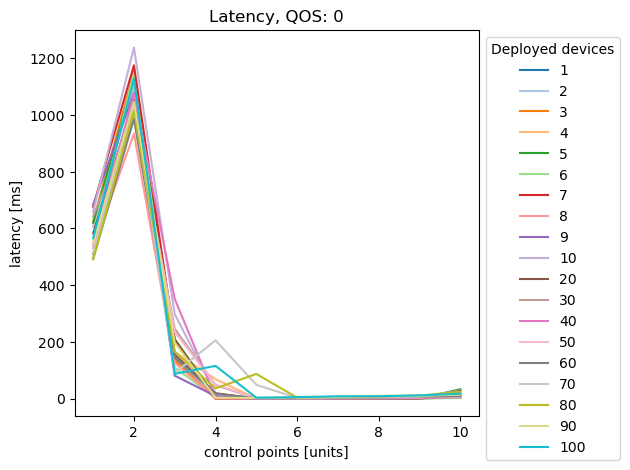
\includegraphics[width=3.5in]{results/mqtt_latency_q0.png}%TODO CABLED
    \label{fig_mqtt_latency_q0_cabled}}
    \caption{\gls{mqtt} latency \gls{qos} 0}
    \label{fig_mqtt_latency_q0}
\end{figure*}

\begin{figure*}[!ht]
    \centering
    \subfloat[]{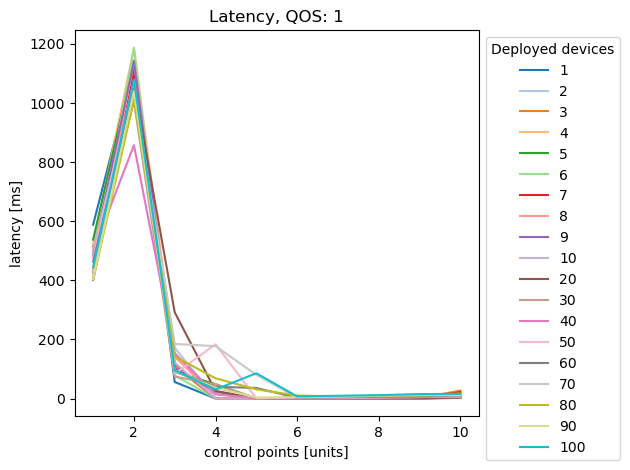
\includegraphics[width=3.5in]{results/mqtt_latency_q1.png}
    \label{fig_mqtt_latency_q1_wireless}}
    \hfil
    \subfloat[]{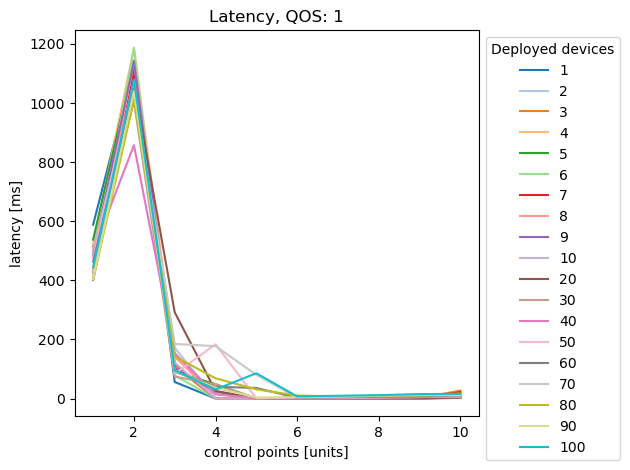
\includegraphics[width=3.5in]{results/mqtt_latency_q1.png}%TODO CABLED
    \label{fig_mqtt_latency_q1_cabled}}
    \caption{\gls{mqtt} latency \gls{qos} 1}
    \label{fig_mqtt_latency_q1}
\end{figure*}

\begin{figure*}[!ht]
    \centering
    \subfloat[]{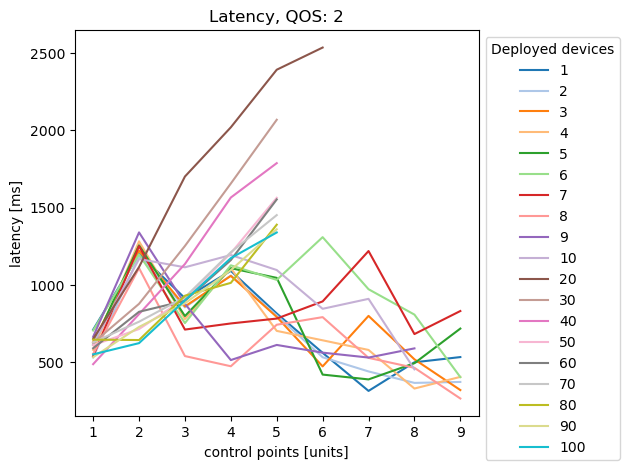
\includegraphics[width=3.5in]{results/mqtt_latency_q2.png}
    \label{fig_mqtt_latency_q2_wireless}}
    \hfil
    \subfloat[]{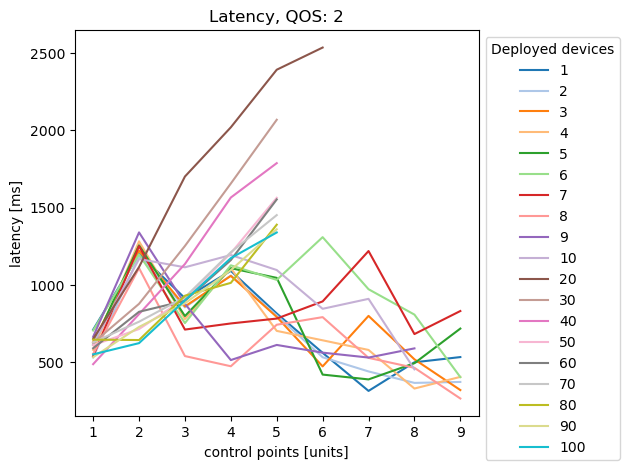
\includegraphics[width=3.5in]{results/mqtt_latency_q2.png}%TODO CABLED
    \label{fig_mqtt_latency_q2_cabled}}
    \caption{\gls{mqtt} latency \gls{qos} 2}
    \label{fig_mqtt_latency_q2}
\end{figure*}

\subsubsection{\gls{mqtt} robustness}
\begin{figure*}[!ht]
    \centering
    \subfloat[]{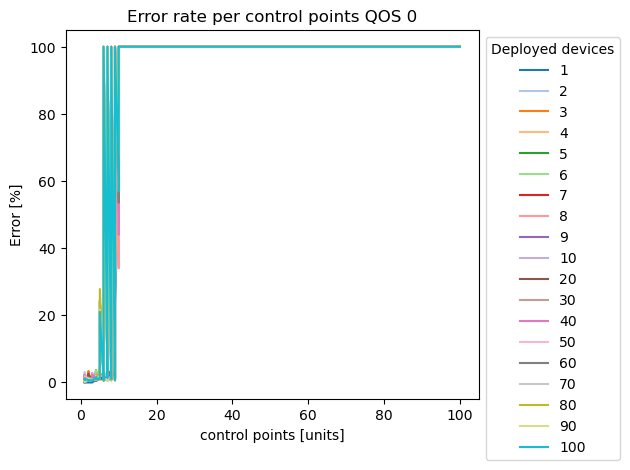
\includegraphics[width=3.5in]{results/mqtt_robustness_q0.png}
    \label{fig_mqtt_robustness_q0_wireless}}
    \hfil
    \subfloat[]{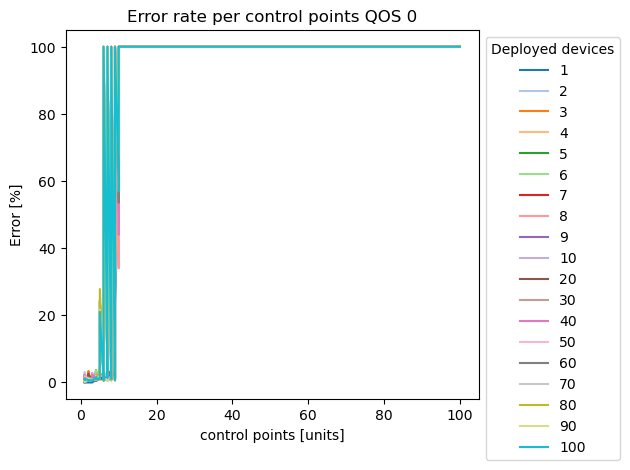
\includegraphics[width=3.5in]{results/mqtt_robustness_q0.png}%TODO CABLED
    \label{fig_mqtt_robustness_q0_cabled}}
    \caption{\gls{mqtt} latency \gls{qos} 0}
    \label{fig_mqtt_robustness_q0}
\end{figure*}

\begin{figure*}[!ht]
    \centering
    \subfloat[]{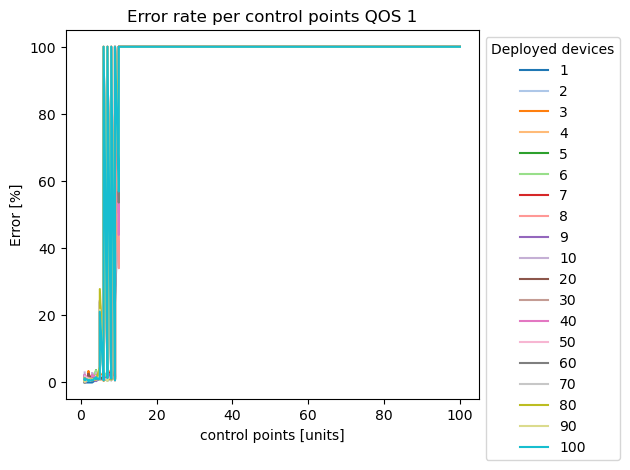
\includegraphics[width=3.5in]{results/mqtt_robustness_q1.png}
    \label{fig_mqtt_robustness_q1_wireless}}
    \hfil
    \subfloat[]{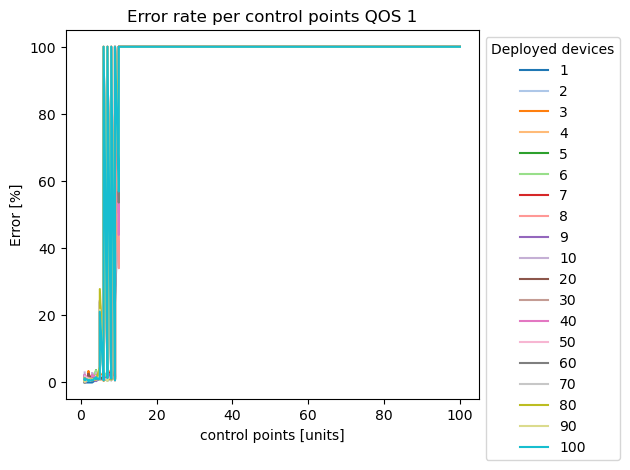
\includegraphics[width=3.5in]{results/mqtt_robustness_q1.png}%TODO CABLED
    \label{fig_mqtt_robustness_q1_cabled}}
    \caption{\gls{mqtt} latency \gls{qos} 1}
    \label{fig_mqtt_robustness_q1}
\end{figure*}

\begin{figure*}[!ht]
    \centering
    \subfloat[]{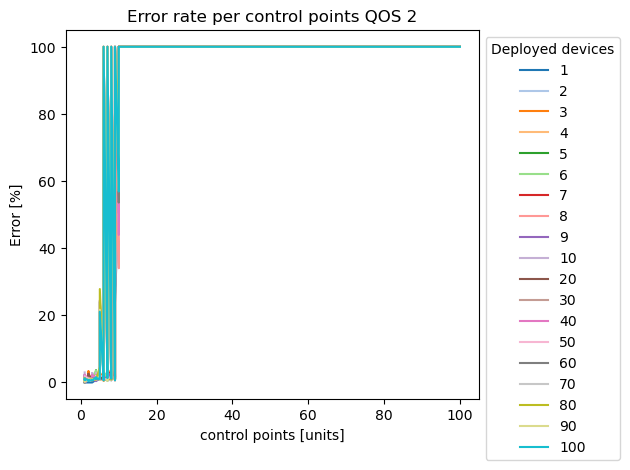
\includegraphics[width=3.5in]{results/mqtt_robustness_q2.png}
    \label{fig_mqtt_robustness_q2_wireless}}
    \hfil
    \subfloat[]{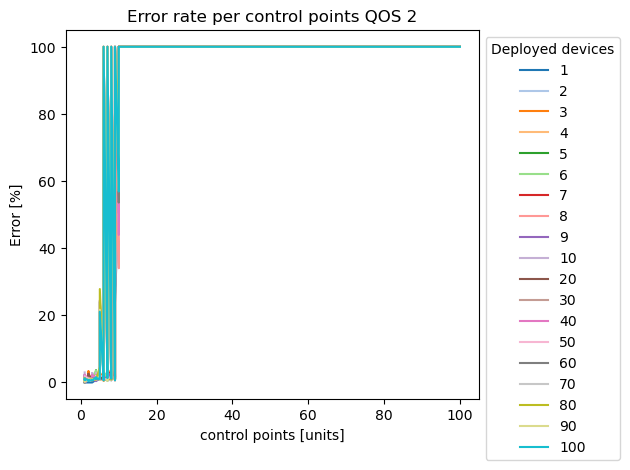
\includegraphics[width=3.5in]{results/mqtt_robustness_q2.png}%TODO CABLED
    \label{fig_mqtt_robustness_q2_cabled}}
    \caption{\gls{mqtt} latency \gls{qos} 2}
    \label{fig_mqtt_robustness_q2}
\end{figure*}

\subsection{\gls{upnp}}
\subsubsection{\gls{upnp} latency}
\begin{figure*}[!ht]
    \centering
    \subfloat[]{
\includegraphics[width=3.5in]{results/upnp_latency.png}
    \label{fig_upnp_latency_wireless}}
    \hfil
    \subfloat[]{
\includegraphics[width=3.5in]{results/upnp_latency.png}%TODO CABLED
    \label{fig_upnp_latency_cabled}}
    \caption{\gls{upnp} latency}
    \label{fig_upnp_latency}
\end{figure*}

\begin{figure*}[!ht]
    \centering
    \subfloat[]{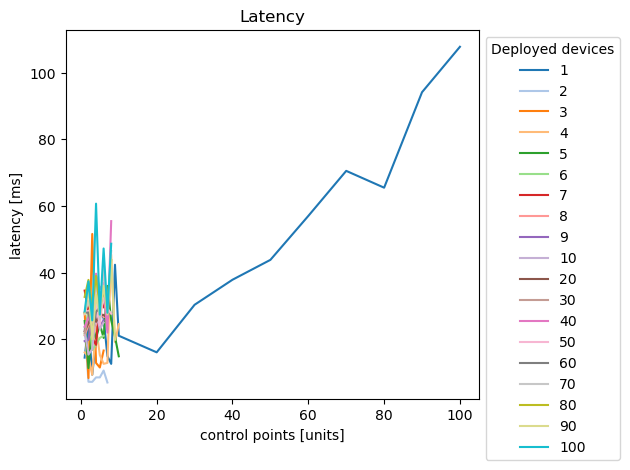
\includegraphics[width=3.5in]{results/upnp_0_latency.png}
    \label{fig_upnp_0_latency_wireless}}
    \hfil
    \subfloat[]{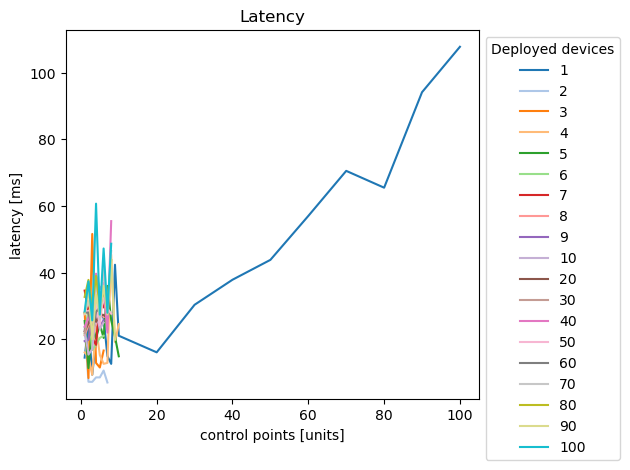
\includegraphics[width=3.5in]{results/upnp_0_latency.png}%TODO CABLED
    \label{fig_upnp_0_latency_cabled}}
    \caption{\gls{upnp} latency with no random delay}
    \label{fig_upnp_0_latency}
\end{figure*}

\subsubsection{\gls{upnp} robustness}
\begin{figure*}[!ht]
    \centering
    \subfloat[]{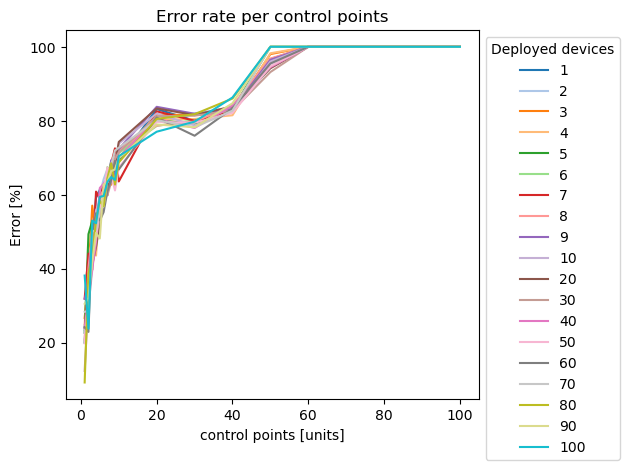
\includegraphics[width=3.5in]{results/upnp_robustness.png}
    \label{fig_upnp_robustness_wireless}}
    \hfil
    \subfloat[]{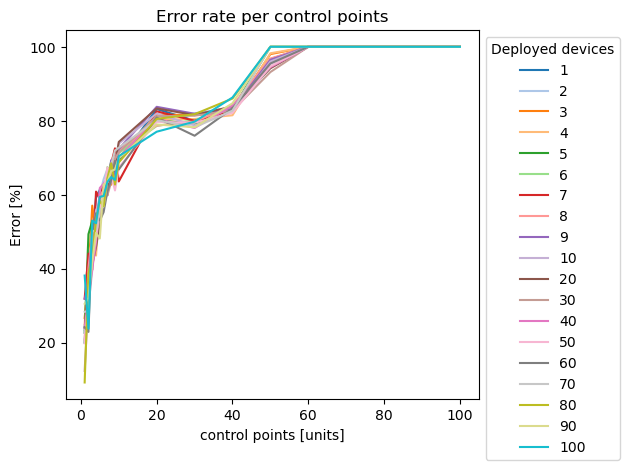
\includegraphics[width=3.5in]{results/upnp_robustness.png}%TODO CABLED
    \label{fig_upnp_robustness_cabled}}
    \caption{\gls{upnp} robustness}
    \label{fig_upnp_robustness}
\end{figure*}

\begin{figure*}[!ht]
    \centering
    \subfloat[]{
\includegraphics[width=3.5in]{results/upnp_0_robustness.png}
    \label{fig_upnp_0_robustness_wireless}}
    \hfil
    \subfloat[]{
\includegraphics[width=3.5in]{results/upnp_0_robustness.png}%TODO CABLED
    \label{fig_upnp_0_robustness_cabled}}
    \caption{\gls{upnp} robustness with no random delay}
    \label{fig_upnp_0_robustness}
\end{figure*}

\bibliographystyle{IEEEtran}
\bibliography{bibliography}

\end{document}


